\documentclass[12pt,letterpaper,final]{report}
\usepackage[utf8]{inputenc}
\usepackage{amsmath}
\usepackage{amsfonts}
\usepackage{amssymb}
\usepackage{amsthm}
\renewcommand\qedsymbol{$\blacksquare$}
\usepackage{enumerate}
\usepackage{hyperref}
\usepackage{pdfpages}
\usepackage{graphics}
\usepackage{graphicx}
\usepackage{tikz}
\usepackage{tikz-qtree}
\usetikzlibrary{automata,arrows, arrows.meta, positioning}
\usepackage[
  backend=biber,
  style=authoryear,
  sorting=nyt          % sort by name, year, title
]{biblatex}
\addbibresource{references.bib}

\author{Jonathan Llovet}

\begin{document}

\fbox{
  \vbox{
    \begin{flushleft}
      Jonathan Llovet \\  % authors' names
      COSC 417 \\  %class
      2026-03-05, 11:59 PM (EST) \\  % date
    \end{flushleft}
    \center{\Large{\textbf{Assignment 4}}}
    %\end{mdframed}
  } % end vbox
} % end fbox

\vspace{0.5cm}


\emph{Practice Examples and Exercises.}  Read Examples 2.3, 2.4, 2.14, 2.16 from the textbook. Do without turning in exercises 2.3, 2.4 (a, d), 2.6 (a,c) (these exercises have solutions in the textbook. Attempt to solve the exercises before reading the solutions).  Some of these exercises may  show up in quizzes and exams.
\bigskip

\textbf{Problem 1.}  Exercise 2.1, textbook Chapter 2. Note: you must present derivations (see bottom of page 102 in the textbook) and also parse trees (see  Fig. 2.1, in the textbook).
\bigskip

The given grammar $G_1$:
\begin{align*}
  E & \to E + T\ \vert\ T      \\
  T & \to T \times F\ \vert\ F \\
  F & \to (E)\ \vert\ a
\end{align*}

\noindent(a) Derivation $E \Rightarrow^* a$

\medskip
\noindent
\begin{minipage}[t]{0.35\textwidth}
  \vspace{0pt}
  \begin{align*}
    E & \Rightarrow T \\
      & \Rightarrow F \\
      & \Rightarrow a \\
  \end{align*}
\end{minipage}%
\hfill
\begin{minipage}[t]{0.6\textwidth}
  \vspace{0pt}
  \centering
  \begin{tikzpicture}
    \Tree
    [.E
        [.T
            [.F
                [.a ]
            ]
        ]
    ]
  \end{tikzpicture}
\end{minipage}

\pagebreak
\noindent(b) Derivation $E \Rightarrow^* a + a$

\medskip
\noindent
\begin{minipage}[t]{0.35\textwidth}
  \vspace{0pt}
  \begin{align*}
    E & \Rightarrow E + T \\
      & \Rightarrow T + T \\
      & \Rightarrow F + T \\
      & \Rightarrow F + F \\
      & \Rightarrow a + F \\
      & \Rightarrow a + a \\
  \end{align*}
\end{minipage}%
\hfill
\begin{minipage}[t]{0.6\textwidth}
  \vspace{0pt}
  \centering
  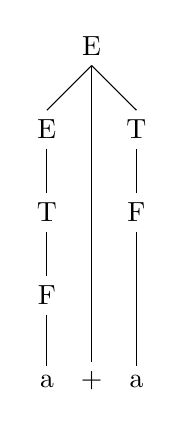
\begin{tikzpicture}
    \Tree
    [.E
        [.E
            [.T
                [.F
                    [.a ]
                ]
            ]
        ]
        [[[[.{$+$} ]]]]
        [.T
            [.F
                [[.a ]]
            ]
        ]
    ]
  \end{tikzpicture}
\end{minipage}

\bigskip
\noindent(c) Derivation $E \Rightarrow^* a + a + a$

\medskip
\noindent
\begin{minipage}[t]{0.35\textwidth}
  \vspace{0pt}
  \begin{align*}
    E & \Rightarrow E + T     \\
      & \Rightarrow E + T + T \\
      & \Rightarrow T + T + T \\
      & \Rightarrow F + T + T \\
      & \Rightarrow F + F + T \\
      & \Rightarrow F + F + F \\
      & \Rightarrow a + F + F \\
      & \Rightarrow a + a + F \\
      & \Rightarrow a + a + a \\
  \end{align*}
\end{minipage}%
\hfill
\begin{minipage}[t]{0.6\textwidth}
  \vspace{0pt}
  \centering
  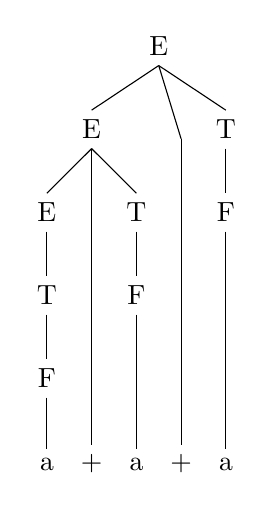
\begin{tikzpicture}
    \Tree
    [.E
        [.E
            [.E
                [.T
                    [.F
                        [.a ]
                    ]
                ]
            ]
            [[[[.{$+$} ]]]]
            [.T
                [.F
                    [[.a ]]
                ]
            ]
        ]
        [[[[[.{$+$} ]]]]]
        [.T
            [.F
                [[[.a ]]]
            ]
        ]
    ]
  \end{tikzpicture}
\end{minipage}

\pagebreak
\noindent(d) Derivation $E \Rightarrow^* ((a))$

\medskip
\noindent
\begin{minipage}[t]{0.35\textwidth}
  \vspace{0pt}
  \begin{align*}
    E & \Rightarrow T     \\
      & \Rightarrow F     \\
      & \Rightarrow (E)   \\
      & \Rightarrow (T)   \\
      & \Rightarrow (F)   \\
      & \Rightarrow ((E)) \\
      & \Rightarrow ((T)) \\
      & \Rightarrow ((F)) \\
      & \Rightarrow ((a)) \\
  \end{align*}
\end{minipage}%
\hfill
\begin{minipage}[t]{0.6\textwidth}
  \vspace{0pt}
  \centering
  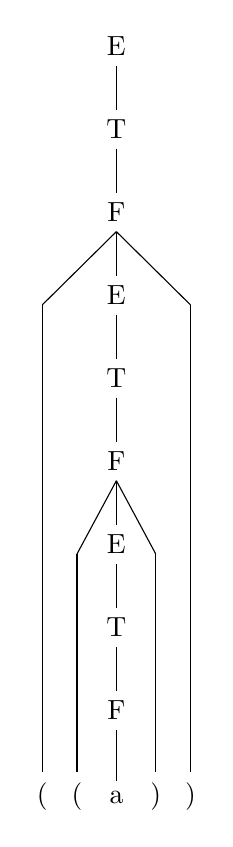
\begin{tikzpicture}
    \Tree
    [.E
        [.T
            [.F
                [[[[[[[.{(} ]]]]]]]
                [.E
                    [.T
                        [.F
                            [[[[.{(} ]]]]
                            [.E
                                [.T
                                    [.F
                                        [.a ]
                                    ]
                                ]
                            ]
                            [[[[.{)} ]]]]
                        ]
                    ]
                ]
                [[[[[[[.{)} ]]]]]]]
            ]
        ]
    ]
  \end{tikzpicture}
\end{minipage}

\pagebreak
\textbf{Problem 2.}  (a)  Give a context-free grammar $G_1$ with $3$ rules  for the language $A_1 = \{0^i 1^j \mid i > j \geq 0\}$.

The grammar $G_1$:

\begin{align*}
  R & \to S             \\
  S & \to 0S1\ \vert\ T \\
  T & \to 0\
\end{align*}

Show a derivation in your grammar of the string $00011$.

\begin{align*}
  R & \Rightarrow S     \\
    & \Rightarrow 0S1   \\
    & \Rightarrow 00S11 \\
    & \Rightarrow 00T11 \\
    & \Rightarrow 00011 \\
\end{align*}

(b)  Give a context-free grammar $G_2$ with $3$ rules for the language $A_2 = \{0^i 1^j \mid 0 \leq  i < j\}$.

The grammar $G_2$:

\begin{align*}
  L & \to M             \\
  M & \to 0M1\ \vert\ P \\
  P & \to 1\
\end{align*}


Show a derivation in your grammar of the string $00111$.

\begin{align*}
  L & \Rightarrow M     \\
    & \Rightarrow 0M1   \\
    & \Rightarrow 00M11 \\
    & \Rightarrow 00P11 \\
    & \Rightarrow 00111 \\
\end{align*}


(c)   Give a context-free grammar $G_3$ for the language $A_3 = \{0^i 1^j \mid i \not=  j\}$. (Note: $A_3$ is the union of $A_1$ and $A_2$.)

The grammar $G_3 = G_1 \cup G_2$:

\begin{align*}
  N & \to L \mid R   \\
  L & \to M          \\
  M & \to 0M1 \mid P \\
  P & \to 1          \\
  R & \to S          \\
  S & \to 0S1 \mid T \\
  T & \to 0
\end{align*}

Show a derivation in your grammar of the strings $00011$ and $00111$.

\noindent
\begin{minipage}[t]{0.45\textwidth}
  \vspace{0pt}
  Derivation $N \Rightarrow^* 00011$
  \begin{align*}
    N & \Rightarrow R     \\
      & \Rightarrow S     \\
      & \Rightarrow 0S1   \\
      & \Rightarrow 00S11 \\
      & \Rightarrow 00T11 \\
      & \Rightarrow 00011 \\
  \end{align*}
\end{minipage}%
\hfill
\begin{minipage}[t]{0.45\textwidth}
  \vspace{0pt}
  Derivation $N \Rightarrow^* 00111$
  \begin{align*}
    N & \Rightarrow L     \\
      & \Rightarrow M     \\
      & \Rightarrow 0M1   \\
      & \Rightarrow 00M11 \\
      & \Rightarrow 00P11 \\
      & \Rightarrow 00111 \\
  \end{align*}
\end{minipage}

\pagebreak

\textbf{Problem 3.}   Give a PDA for the language $L = \{w \in \{0,1\}^* \mid w = w^R\}$ (the language of all binary strings that are palindromes). (Hint: Do something similar to Example 2.18 in the textbook, the difference being that you also need to handle strings having odd length.)

You must give an informal description (in English) of your PDA, and the diagram (your explanations should be in the style of the Example 2.18 from the textbook).

\begin{center}
  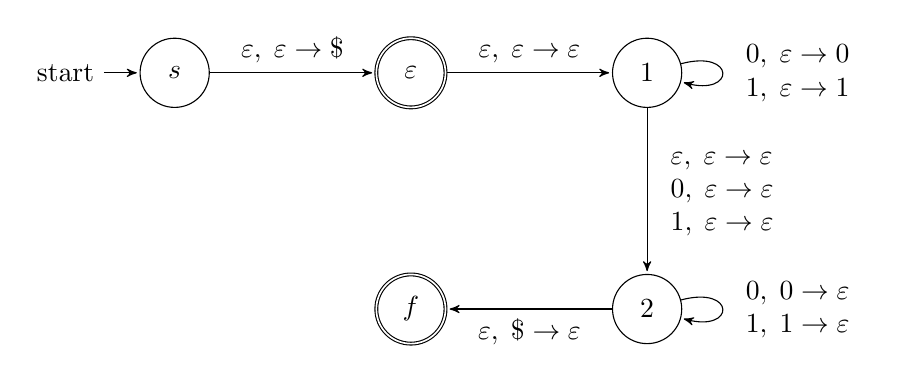
\begin{tikzpicture}[>=stealth',shorten >=1pt,auto,node distance=3cm]

    \node[initial, state] (s) {$s$};
    \node[state, accepting] (e) [right of=s] {$\varepsilon$};
    \node[state] (1) [right of=e] {$1$};
    \node[state] (2) [below of=1] {$2$};
    \node[state, accepting] (f) [left of=2] {$f$};

    \path[->]
    (s) edge node {$\varepsilon,\; \varepsilon \to \$$} (e)
    (e) edge node {$\varepsilon,\; \varepsilon \to \varepsilon$} (1)
    (1) edge [loop right] node[right] {$\begin{array}{l} 0,\; \varepsilon \to 0 \\ 1,\; \varepsilon \to 1 \end{array}$} (1)
    (1) edge node[right] {$\begin{array}{l} \varepsilon,\; \varepsilon \to \varepsilon \\ 0,\; \varepsilon \to \varepsilon \\ 1,\; \varepsilon \to \varepsilon \end{array}$} (2)
    (2) edge [loop right] node[right] {$\begin{array}{l} 0,\; 0 \to \varepsilon \\ 1,\; 1 \to \varepsilon \end{array}$} (2)
    (2) edge node {$\varepsilon,\; \$ \to \varepsilon$} (f)
    ;
  \end{tikzpicture}
\end{center}

\begin{enumerate}
  \item The PDA starts by placing $\$$ on the stack while transitioning from state $s$ to state $\epsilon$, which is accepting, since the empty string is the same as its reverse.
  \item From state $\epsilon$ it does an epsilon transitions to state $1$, with no modification to the stack. Now it will start handling non-empty strings.
  \item In state $1$, the PDA consumes the first half of even-length strings, the first $\frac{n-1}{2}$ characters of odd-length strings. As it consumes each character, it pushes the same character on the stack.
  \item In the case that the string is of even length $n$, the transition from state $1$ to state $2$ is along the epsilon transition after the first $n/2$ characters have been consumed.
  \item In the case that the string is of odd length $n$, the transition from state $1$ to state $2$ is along the corresponding labeled transition on the middle character of the string, the ${\frac{n-1}{2}+1}^{st}$ character, but with no modification of the stack. This allows the middle character to be consumed and then proceed using the same strategy as we use for even-length strings.
  \item Once in state $2$, the PDA consumes the remaining characters in the input, popping the same character off the stack as it is read from the input.
  \item If the input and the stack are exhausted at the same time, then the PDA will proceed along an epsilon transition to accepting state $f$, reading the special symbol $\$$ indicating the stack is empty. Otherwise, if the stack and the input are not consumed at the same time, the string will be rejected.
\end{enumerate}


\bigskip
\textbf{Problem 4}  A prefix of a string $x$ is a string $y$ such that there is $z$ with $x=yz$. For instance, the string $1011$ has prefixes $\epsilon, 1, 10, 101, 1011$.  Show that if $L$ is a regular language, then
\[
  \mathsf{pref}(L) = \{y \in \Sigma^* \mid y \textrm{ is a prefix of a string in $L$ } \}
\]
is also regular. In your proof, consider the state diagram (the graph) of a DFA that recognizes $L$ and indicate how to modify it to obtain a DFA or an NFA that recognizes  $\mathsf{pref}(L).$

{\bf Proof:} Since $L$ is regular, there is a DFA that recognizes $L$. For every string $w \in L$, the sequence of characters $w_1, w_2, \ldots, w_k$ induces a path from the start state $q_0$ to an accepting state $q_f$. To transform the DFA into an NFA that accepts $\mathsf{pref}(L)$, we will strategically add $\epsilon$ transitions, similar to the modifications we made for showing closure properties of NFAs. First, create a new accepting state $q_{accept\_prefix}$. For all paths that are induced by reading strings $w \in L$, there is a sequence of states traversed between the reading of $w_1$ and $w_k$, namely $q_0 \Rightarrow q_f$. For each such path, place an $\epsilon$ transition from each state $q_i$, where $0 \le i \le k$, to $q_{accept\_prefix}$. This will mean that while reading a string $w \in L$, any state that can be entered will be able to be accepted by performing the $\epsilon$ transition to $q_{accept\_prefix}$. Because of this, any prefix of $w$ is accepted, which is $\mathsf{pref}(L)$, QED.

An alternative way to approach this construction is to similarly observe that there is a DFA for the given regular language $L$. Call that DFA $M$. Perform a minimization of $M$, so that there are no unreachable states, there are no dead states, and none of the states are indistinguishable. This would result in a DFA $M'$ that consists of a unique set of paths induced from the start state to accepting states. Similarly to above, create a new state $q_{accept\_prefix}$ that will serve as the only accepting state of $M'$, and create an $\epsilon$ transition from all of the other states to $q_{accept\_prefix}$. At any point in reading a string $w$, it will be possible to transition to the state $q_{accept\_prefix}$ along an $\epsilon$ transition, meaning that every prefix of $w$ can be accepted, which is what we wanted.

\qed

\end{document}
